%\VignetteIndexEntry{Short overview of package sdcMicro}
\documentclass[12pt]{article}
%\usepackage{a4,graphicx,fancyhdr, vmargin,luxstyle}
\usepackage{a4,graphicx,fancyhdr, vmargin, psfig, texstyle}
\usepackage{natbib}
\bibliographystyle{plain}
 
\usepackage{c:/Programme/R/R-2.5.0/share/texmf/Sweave}
\begin{document}
\begin{flushleft}
  {\LARGE\bf {\tt sdcMicro}: a new flexible {\bf R}-package for the generation of anonymised microdata:  \\[2mm]Design issues and new methods } 
  \vspace{1.0cm}
  
  Matthias Templ$^*$%, Second Author$^{**}$
 
{\small
\begin{description}
\item $^* \;$ Department of Methodology, Statistics Austria, Guglgasse 13, 1110 Vienna, Austria.
    (matthias.templ@statistik.gv.at) and \\
\item $^{*}\;$    Department of Statistics and Probability Theory, Vienna University of Technology, Wiedner Hauptstr. 8-10, 1040 Vienna, Austria. 
    (templ@tuwien.ac.at)
%\item $^{**}\;$ Another University, Another Institute, Anotherland,
%  (sauthor@another.university.org)
\end{description}
}
\end{flushleft}
\vspace{1cm}


\noindent {\bf Abstract}.
{\small Data protection specialists need flexible software tools for the exploratory use of protection methods to generate high quality confidential data. Microdata protection is widely used and is often the only possible way to provide data to both researchers and users. In this paper we present a methodological and computational framework for the generation of anonymised microdata and give insights to the developed {\bf R}-package {\tt sdcMicro}. This package may become the standard software for microdata protection since it is very flexible, easy to use and contains all popular methods, plus some new ones. The package can also be used for comparison of methods and of original versus perturbed data not only by measuring information loss but also by various comparison plots.
}

%%%%%%%%%%%%%%%%%%%%%%%%%%%%%%%%%%%%%%%%%%%%%%
\section{Motivation}
Nowadays there are various methods for dealing with confidential microdata developed to make such data accessible to researchers and users.
Roughly speaking, these methods can be clustered into 3 categories: 
\begin{itemize}
  \item[(i)] Remote Access based on the idea of hidden data and checked outputs.
  \item[(ii)] Remote Access based on the idea of a free view of the data without the possibility to download the data.
  \item[(iii)] perturbed microdata publicity as {\it public} or {\it scientific use files} or different variants between public and scientific use files.
\end{itemize}

In the following there is a short motivation of point (iii) since many researchers do not see a future in this point (iii) and therefore do not see the necessarity for a (new) software on microdata protection.

Regarding (i) researchers can apply models on data which can not be seen or where data and particularly outliers are perturbed \citep[see e.g. in]{Heitzig06} but they can apply models. This approach is often called {\it confidential preserving model servers}. But it is the results of a models which are the objects of interest not the underlying data \citep{Steel05}. Considering a {\it Remote Execution} framework these results are checked by the census staff and, for example, in case of regression analysis synthetic residuals are often provided. But then, you see synthetic residuals based on residuals from really worst estimates because of using least squares regression on data which, naturally, includes outliers. Furthermore, you would never have the ability to find a good model without applying the whole range of diagnostic tools on robust estimates. This is in contradiction to \cite{Heitzig05} and others (e.g. \cite{Steel05}) because for such robust estimates it is improbably to provide synthetic residuals (because you always see large or heavy perturbed residuals/outliers), for example, and there is no method  available for the detection of leverage points. It is also well known in robust statistics literature that you need robust methods for the detection of outliers which are essential and which cannot be provided. We can conclude that model servers are not compatible with a modern statistical world unless the underlying data is of a multivariate normal distribution or can be transformed into one which turns out to be unrealistic for real complex data. Concluding that, model servers are not compatible with a modern statistical world with the expection the underlying data is of a or can be transformed to a multivariate normal distribution which is unrealistic for real complex data. 

In the second approach (ii) researchers may look at the data and can choose a suitable method for analysing the data, but it is not possible to download the data in any way (for applications in (ii) see e.g. \cite{Hundepool05oh} or \cite{Borchsenius05}). Remote access can only partially be applied in some countries depending on the discipline from which the data originates. This is due to different legacy for data coming from different disciplines. In Austria, for example, only microdata protection is reasonable for official statistics because of the legal situation which prohibits a view on ``original'' data.

In (iii) users and researchers have access to perturbed data. In this paper we will show that such a perturbation can be easily performed with newly developed and extremely flexible software package by minimizing information loss and re-identification. 

In addition to that, we will also concentrate on the design of this new package for microdata protection and illustrate the open source philosophy of this project.
 
%Some people might see the future of dealing with confidential microdata in confidentiality preserving model servers or in remote access facilities. For the first approach, roughly speaking, researchers can apply models on data which can not be seen and the results of the models will be checked by the census staff. So, the results of a model is the object of interest not the underlying data. This approach makes only sense when the data originates from a multivariate normal distribution, but it is not compatible with a modern statistical world and real data with outliers and complex structures.
%In the second approach, remote access, researchers can look at the data and can choose a suitable method for analysing the data, but it is not possible to download the data. Because of the legal situation in many countries including Austria together with the lack of interest because of additional expenditure for remote access I suppose that remote access will only partially successful applied in some countries depending also on which discipline the data originates, because of different legal laws for data coming from different disciplines. Regarding to all these aspects a new open-source software initiative for microdata protection may be of great interest. 


%%%%%%%%%%%%%%%%%%%%%%%%%%%%%%%%%%%%%%%%%%%%%%
\section{Using {\bf R} for SDC}

{\bf R} \cite{R07} is an open source high-level statistical computing environment subjected to the General Public License and therefore freely available and expendable. Furthermore, {\bf R} has become the standard statistical software and thousands of people are involved in the development of {\bf R} both at universities and companies. More than 1000 add-on packages have been built in the last years.

In the following the usefulness of {\bf R} related to SDC is presented.
The most important and most essential feature of a software for SDC is the reproducibility of results. The most effective way of anonymising microdata is by doing the anonymisation steps in an explorative and in some sense iterative way, since we can apply various methods on various variables with different parameters producing different effects on the data and while looking for sufficient anonymisation of the data with respect to low information loss. Therefore, we must have the ability to reproduce any step of the anonymisation process easily. This is fulfilled by running a script with all the commands included. It is then easy to change and adapt this script and get all the new results ``in real time''. Of course, this is fulfilled by many software tools, but the real advantage of using {\bf R} is that we can interactively ``play'' with the data, i.e. we have access to all the objects in the workspace of {\bf R} any time and can change, display or apply operations on it on the fly. This is very useful during the anonymisation of data and a quite different concept than to write a ``batch file'' which can then be executed.  

In addition to that, we recommend the use of a powerful easy-to-grasp visualization tools to see the effect of the anonymisation on the data instead of computing various measures of information loss (see e.g. in \cite{Templ06}).

But dynamical reports can also be used for documenting the anonymisation  when using {\bf R} in combination with {\tt Sweave} (\cite{Leisch02}). Reports can then be generated very effectively and quickly for particular steps in the production process.

Since many different possible data formats are used by users it is very comfortable to have the opportunity to import and export data formats from data base software and statistical software like {\tt SPSS}, {\tt SAS}, {\tt Stata}, {\tt DBF}, {\tt Excel}, {\tt ASCII}, and many more. Sometimes it is also useful to run the anonymisation tools via batch mode, which can be easily derived with package {\tt sdcMicro} \citep{TemplR07}.

It is also very important to provide a software for SDC which is platform independent and works on all common operating systems.

All these things are supported when using {\bf R}.

An important and essential feature of any software dealing with data is the reproducibility of results. An advantage of a command line interface (CLI) like in {\bf R} is that any result can be reproduced very easily. Furthermore, all the code is open-source and one can have a detailed look at the code in each of the steps of the microdata protection procedure for any method. Also very important is the reproducibility of results when applying different algorithms for SDC on data and doing a validation and comparison of these different results.

{\bf R} has very powerful graphical tools implemented and one can generate simple and complex user-defined graphics easily. This is very important since mostly it is better to show perturbation effects or other effects resulting from the protection process with suitable plots as with some measures of information loss (see e.g. also in \cite{Templ06}).

In combination with \LaTeX \ someone can produce dynamical reports, where \LaTeX -code and {\bf R}-code can be written and executed in/from one document with the help of {\tt Sweave} \cite{Leisch02}. Of course, one can also standardise such dynamical reports to get automatically all the results from any data in a standardised format. Such reports can then generated very effective and could save time for particular steps in the production process.

Nearly all common data formats from database software and other statistical software like SPSS, SAS, STATA, MINITAB, DBF, \ldots can be imported. Furthermore, there are also procedures available to export the data in most of these data formats. 

\section{Design Goals of Package {\tt sdcMicro}}

When perturbing numerical data the optimal perturbation method depends strongly on the multivariate structure of the data. Therefore, a flexible tool with which one can try out various methods and easily compare the methods is necessary. Even when trying out different global recordings on variables or when playing on some parameters from certain methods a flexible tool and easy to grasp comparison plots and additional evaluation tools are necessary.

For {\bf R} users it is not natural to use a GUI and this might be the main reason why a GUI is only partially implemented for {\it sdcMicro} till now. But, of course,  it is  possible to create a GUI in top of the existing code for {\it sdcMicro}, if there will be a demand for this, since with {\bf R} one can produce powerful GUI's, e.g. with the {\it Rtcltk} package. Nevertheless, the design of the package allows an easy use and not only one of the numerous users ask for a GUI until now.

One can also run the package via batch mode. Furthermore, one can also run directly from {\bf R} any other software which might be also sometimes useful.



%\section{Design Goals}

The advantages of an object-oriented programming language become apparent in the {\tt scdMicro} package.
However, the methods and class approach from {\bf R} is not a class-oriented programming language (like {\tt C} or {\tt Java}) but a richer one as it is a function- and class-oriented programming language. 

In {\bf R} everything is an object and every object is related to a specific class. The class of an object determines how it will be treated and generic functions perform either a task or an action on its arguments specific to the class of the argument itself. The class mechanism offers the programmer the facility of designing and writing generic functions for special purposes which is extensively used in {\it sdcMicro}. Nearly all functions, e.g. the one for the individual risk methodology or the frequency calculation, produce objects from a certain class. Different {\it print}, {\it summary} and {\it plot} methods are provided for each of these objects depending on their class. {\tt plot(ir1)} produces a completely different result than {\tt plot(fc1)} assuming that the objects {\tt ir1} and {\tt fc1} are objects from different classes, i.e. resulting from different functions in package {\it sdcMicro}. \\
This object-oriented approach allows a simple usage of the package for any user, independently of the proficiency in {\bf R}. Furthermore, users can try out different methods with different parameters and they can easily compare the methods with the implemented summary and plot methods.\\


Note that no metadata management needs to be done by the user, even not after importing the data into {\bf R}. You can apply the methods directly on your data sets or on objects for certain classes. At first you must only determine which of the variables are the key variables, the weight vector and the numerical ones. \\
An online documentation is included in the package containing all explanations on all input and output parameters. Furthermore, various examples are included for each of the functions. These examples can be easily executed by the users.

To be able to deal with large data sets extensive computational calculation steps are implemented in {\tt C++} and included in {\bf R} via the {\tt R/C++} interface.
The calculation of the frequency counts is one of the most critical calculation steps regarding to the computation time. Figure (\ref{time}) shows the calculation time carried out by an one year old personal computer\footnote{Intel x86 based system with 3Ghz and 1 GB memory} with Windows XP operating system. The computation time can not be shown in this figure because it turns out to be too large when using loops in {\bf R} for the calculation of the frequency counts because it is too large. Only when using functions in {\bf R}, which are said to be implemented in {\tt C} or {\tt Fortran}, it is possible to calculate the frequency counts with up to 6 key variables by using this relatively small data set with only 4000 observations. This is not possible for the $\mu$-Argus system (\cite{Hundepool06mu}, version 4.1.0) which runs out of memory with 5 or more key variables. The developed {\tt R/C++} can also handle a very large number of key variables\footnote{to choose such a large number of key variables is, of course, not always meaningful.} in reasonable time even for much larger data sets than the $\mu$-Argus test data set. In Figure (\ref{time}) you can easily see that the computation time is always less than 1 second for this small data set and it is also low for larger data sets. 

\begin{figure}
\begin{center}
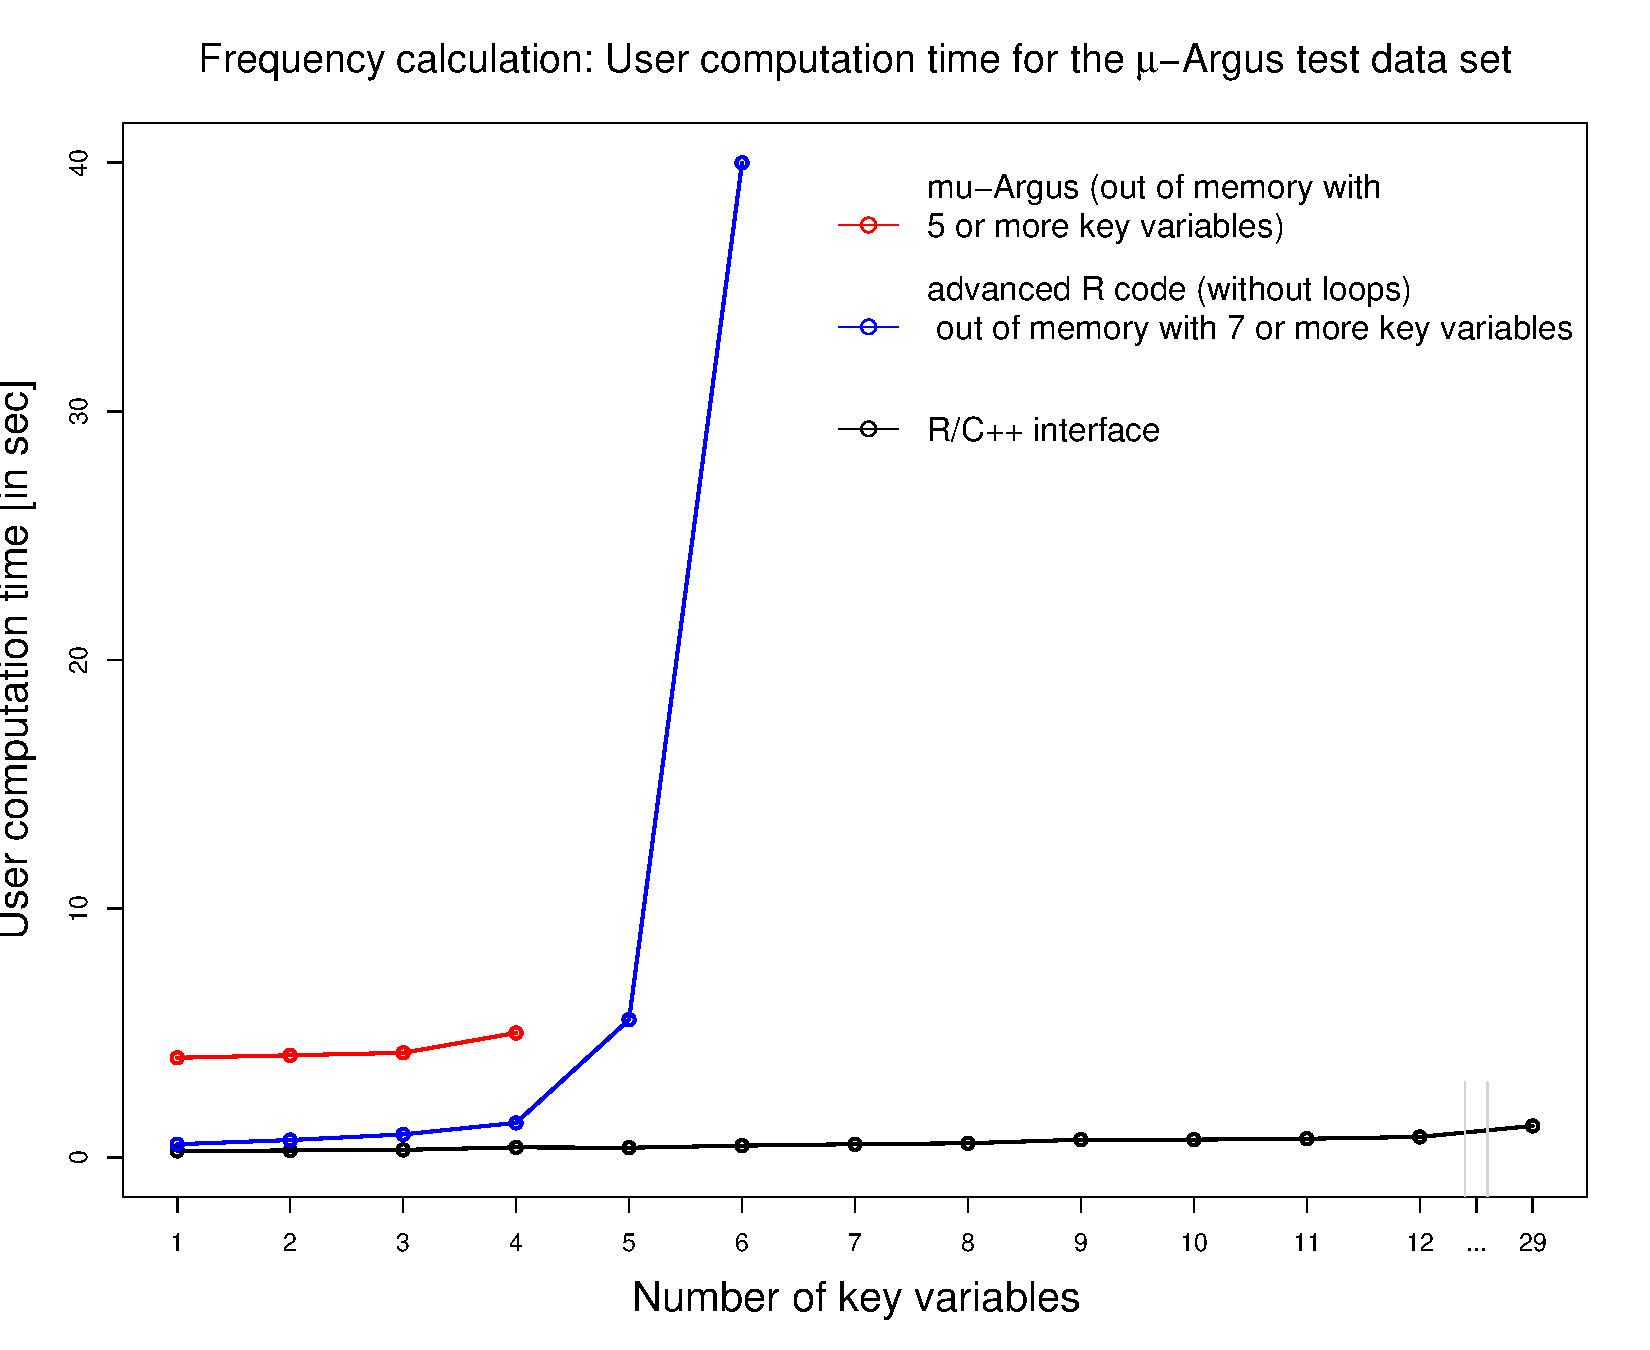
\includegraphics{sdcMicroPaper-001}
\end{center}
%\vspace*{-3cm}
\end{figure} 


\section{Implemented Methods and Data}

Methods like global recoding, local suppression and the individual risk methodology (see e.g. in \cite{Franconi04}), top- and bottom-coding, PRAM (\cite{Kooiman97}), more than 10 microaggregation methods (mdav, pca-methods, robustified pca-methods with fast algorithms and clustering, individual ranking, methods based on robust Mahalanobis distances, \ldots) (more information on these methods and on microaggregation can be found in \cite{Templ06}, \cite{Anwar93}, \cite{Elliot05}, \cite{Defays93}, \cite{Defays98}, \cite{Domingo02}), rank swapping \cite{Dalenius82}, 5 well known adding noise methods (see e.g. in \cite{Brand04}) including ROMM \citep{Ting05} and various other methods are implemented. There is also a method for fast generation of synthetic data included \cite{Sanz04} with which multivariate normal distributed data can be generated regarding to the covariance of the original data, but, of course, this does not reflect the distribution of real complex data. Further methods will be implemented in near future (see below in section {\it Future Developments}).

Several test data sets are implemented in the package. There are some very small test data sets which used by other authors for demonstration in the past. The test data set from $\mu$-ARGUS \cite{Hundepool06mu} can also be used as well as the test data sets from the CASC project \citep{HundepoolCASC04}. 

\subsection{New Methods}
\label{new}

Some new algorithms for microaggregation are proposed and implemented in package {\tt sdcMicro}. 
A simple approach is to cluster the data at first and then sort the data in each group by the most influential variables in the groups or by sorting the observations in each group by the first robust principal component using e.g. the MCD-estimator \citep{Rousseeuw84}. 

We proposed a new algorithm for microaggregation called RMDM ({\bf R}obust {\bf M}ahalanobis {\bf D}istance based {\bf M}icroaggregation where MDAV \citep{Domingo02} is adapted in the following way:
\begin{itemize}
  \item[1.] Compute the robust center of the data. This can be the $L_1$-median or the coordinate-wise median.
  \item[2.] Consider the most distant observation $x_r$ to the robust center using robust Mahalanobis distances. The MCD-Estimator can be used to calculate the robust covariance matrix that is needed for the calculation of the robust Mahalanobis distances.
  \item[3.] Find the most distant observation $x_s$ by calculating robust Mahalanobis distances with the center in $x_r$.
  \item[4.] Choose $k-1$-nearest neighbors from $x_r$ and also from $x_s$ using robust Mahalanobis distances computed with center $x_r$ and center $x_s$. Aggregate $x_r$ and its $k-1$ nearest neighbors with an average as well as $x_s$ with their $k-1$ nearest neighbors. The average can be the arithmetic mean but also robust measures of location.
  \item[5.] Take the previous dataset minus the aggregated data from the last step as a new dataset  and continue with (1.) until all observations are microaggregated.
\end{itemize}

Note, that there are special rules at the end of the algorithm which are described in \cite{Domingo02}. 
This proposed algorithm is more natural than the original MDAV algorithm since we deal with multivariate data taking the covariance structure of the data into account. For larger data sets usual distances can be chosen to find the nearest neighbors in item (4.) of the algorithm (we name this adaption of the algorithm RMDM2). These distances must be calculated only once at the beginning of the algorithm. 

Robust versions of principal component methods for microaggregation are implemented, too.

The {\it clustpppca} and the {\it RMDM2} algorithms for microaggregation worked best for most of the data sets (like the Tarragona data set from the CASC project (see section \ref{Tour})). %For most of the data sets (like the Tarragona data set) the {\tt clustpppca} algorithm performs best (see also the examples in section (\ref{Tour})). 
The {\it clustppca} algorithm is described in \cite{Templ06}. 

Top and bottom coding can be replaced by (multivariate) outlier detection via robust statistics. Only those observations are recoded/perturbed which are outliers and therefore of high re-identification risk. Such a method is included as an adding noise procedure.


\section{A Small Tour in sdcMicro}
\label{Tour}

Within the limitation of pages only a small tour in {\it sdcMicro} can be done excluding most of the graphical results and some steps of recoding variables. Comments are marked with \#, the output from {\bf R} with {\bf R}. For further details, please have a look at the examples and documentation which are included in package {\it sdcMicro}. 

Supposing you have already downloaded and installed {\bf R} and have also installed package {\tt sdcMicro}, which can be installed directly from {\bf R} or downloaded directly from {\it http://cran.r-project.org/src/contrib/Descriptions/sdcMicro.html}, you can load both the package and the data and print\footnote{{\tt xtable()} produces a \LaTeX-styled print output. } the first seven columns and the first four rows of the data with the following command in {\bf R}:

\begin{footnotesize}
\begin{verbatim}
library(sdcMicro); data(free1); xtable(free1[1:4, 1:8])
\end{verbatim}
\end{footnotesize}

% latex table generated in R 2.5.1 by xtable 1.5-1 package
% Fri Oct 05 14:18:33 2007
\small
% latex table generated in R 2.5.1 by xtable 1.5-1 package
% Fri Oct 05 14:19:34 2007
\begin{center}
\begin{tabular}{rrrrrrrr}
  \hline
 & REGION & SEX & AGE & MARSTAT & KINDPERS & NUMYOUNG & NUMOLD \\
  \hline
1 & 36.00 & 1.00 & 43.00 & 4.00 & 3.00 & 0.00 & 0.00 \\
  2 & 36.00 & 1.00 & 27.00 & 4.00 & 3.00 & 0.00 & 0.00 \\
  3 & 36.00 & 1.00 & 46.00 & 4.00 & 1.00 & 0.00 & 0.00 \\
  4 & 36.00 & 1.00 & 27.00 & 4.00 & 1.00 & 0.00 & 0.00 \\
   \hline
\end{tabular}
\end{center}
\normalsize


For this demonstration the $\mu$-Argus test data was chosen but you can simply use another data set from the package or your own data. 

In the following, the frequency counts are calculated as described in \cite{Capobianchi01} and allocated to object {\tt fr1} which is now automatically of class {\tt freqCalc}. Several methods are available for this class. Object {\tt fr1} can then be used as an input for the individual risk computation. A new object {\tt ir1} will be produced which is of class {\tt indivRisk}. Several methods are again available for this class and, for example, function {\tt plot} will automatically know which plot method must be used. Figure (\ref{risk}) is generated by this plot method. The implementation of this plot method for individual risk methods is quite similar as in $\mu$-Argus. 

\begin{footnotesize}
\begin{verbatim}
fr1 <- freqCalc(free1, keyVars=1:3, w=30)
rk1 <- indivRisk(fr1)
class(rk1)
R> [1] "indivRisk"
methods(class = indivRisk)
R> [1] plot.indivRisk  print.indivRisk
plot(rk1)
\end{verbatim}
\end{footnotesize}

The script shown above can easily be adapted  (exclude the {\bf R} results), e.g. 
%By using a script with the R commands included one can easily adapt the script shown above (which the R results), e.g. 
by adding the function {\tt globalRecode()}. {\tt globalRecode()} recodes several
categories of a variable into less categories or discretize a numerical variable. So, this function checks the class of the variable and does the recoding based on the class of the variable. But you still have the ability to manipulate your data in a explorative way. You might try out recoding a variable to observe the influence of your recoding on the frequency count calculation and the individual risk computation. Note that you can easily reproduce all your steps easily either by running a part of your script or the whole script. 

After minimising the re-identification risk you can apply local suppression (function {\tt localSupp()}) on object {\tt indivf} and {\tt fr1} to delete the last unsureness about risky observations and make then use of the implemented print and summary methods. But, also global recoding and local suppression can also be used in an alternated manner, of course.

\begin{figure}
\begin{center}
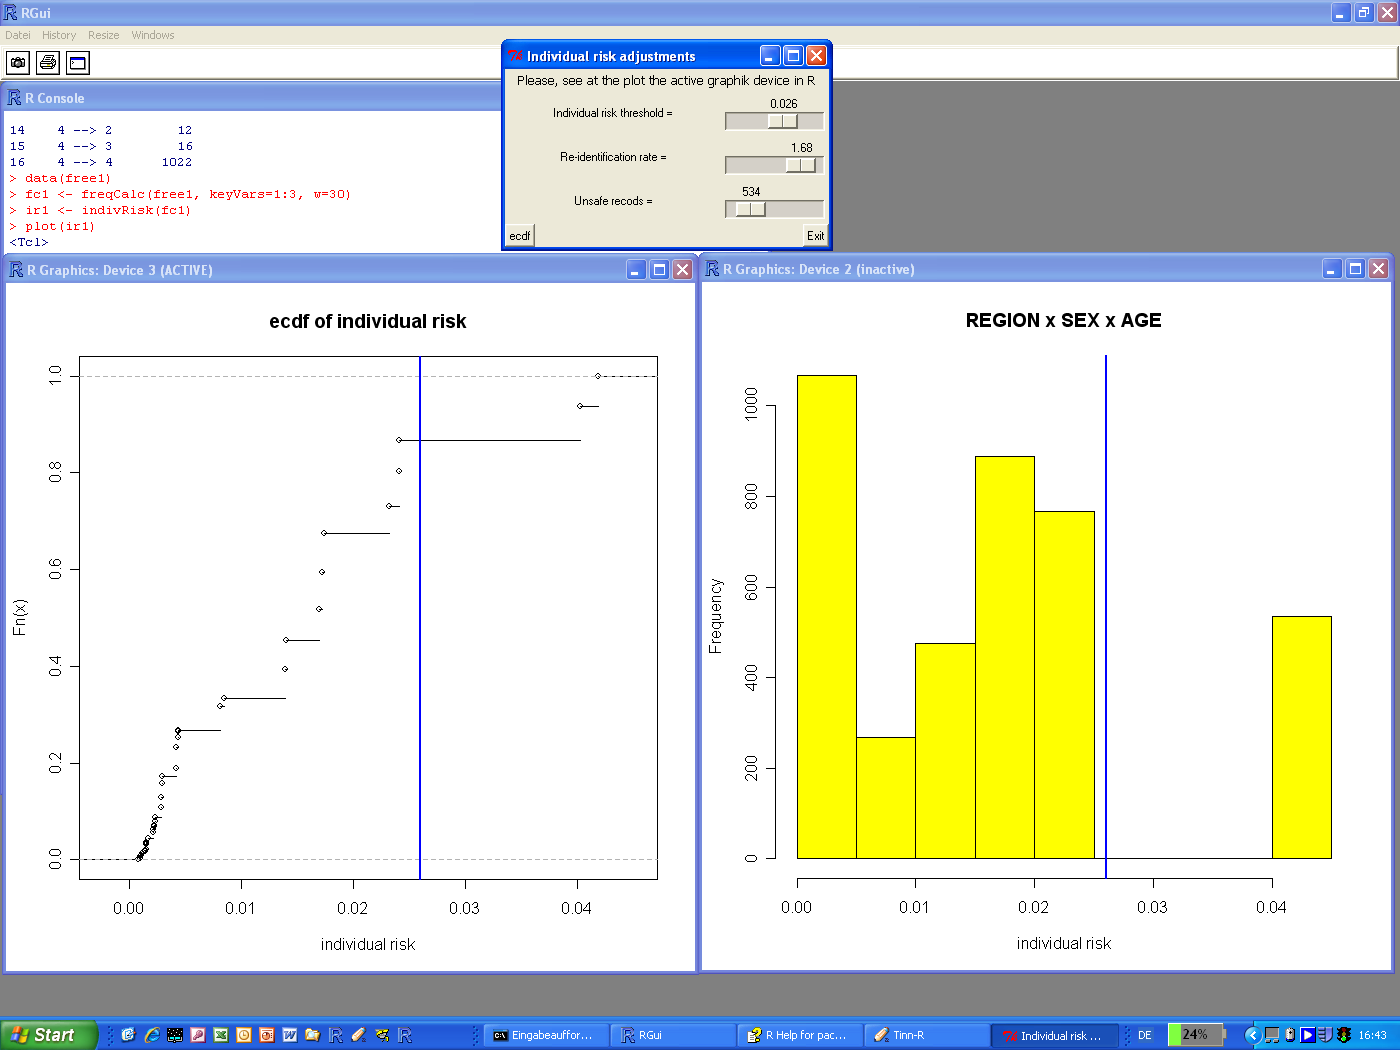
\includegraphics[width=12cm]{risk2.PNG}
\caption{Individual risk for the first 3 variables of the $\mu$-Argus test data set. In the upper region of the figure you will see a helpful slider which is directly linked with the graphics.}
\label{risk}
\end{center}
%\vspace*{-3cm}
\end{figure} 

In addition to that, you can simply microaggregate numerical variables with more than 10 different methods. Furthermore, you can also use rank swapping and adding noise methods. There are a lot of comparison plot methods available to compare the perturbed data and the original data. You can also easily compare the different methods themselves. We will show this on another data set, the {\it Tarragona} data set\footnote{http://neon.vb.cbs.nl/casc/testsets.html}, because the $\mu$-Argus test data does include faked numerical variables which follow a multivariate uniform structure without correlations between the variables.

Microaggregation and a comparison of different methods with various measures of information loss can be done in the following way:

\begin{footnotesize}
\begin{verbatim}
m1 <- microaggregation(Tarragona, method="onedims", aggr=3) # individual ranking method
# now you can use some comparison plots... (see examples of package sdcMicro)
summary(m1) # or the implemented print and summary methods (suppressed)
xtable(valTable(Tarragona, method=c("addNoise: correlated2", "swappNum", "simple",
"onedims", "pca", "mdav", "clustpppca"))[,c(1,2,3,5,6,7,12)]) # measures of inf. loss 
\end{verbatim}
\end{footnotesize}

% latex table generated in R 2.5.1 by xtable 1.5-1 package
% Thu Oct 18 13:15:04 2007
%\begin{table}[ht]
\begin{center}
\begin{tabular}{rlrrrrrr}
  \hline
 & method & amean & amedian & devvar & amad & acov & apcaload \\
  \hline
  1 & addNoise: correlated2 & 0.09 & 3.20 & 0.18 & 5.89 & 0.09 & 8.97 \\
  2 & swappNum & 0.20 & 0.13 & 9.10 & 0.23 & 4.55 & 28.75 \\
  3 & simple & 0.00 & 3.50 & 3.62 & 1.11 & 1.81 & 20.69 \\
  4 & individual ranking & 0.00 & 0.02 & 13.71 & 0.03 & 6.85 & 19.45 \\
  5 & pca & 0.00 & 2.62 & 2.77 & 1.10 & 1.39 & 12.99 \\
  6 & clustpca & 0.00 & 2.34 & 2.69 & 1.11 & 1.35 & 11.72 \\
  7 & mdav & 0.00 & 4.18 & 3.44 & 1.84 & 1.72 & 8.76 \\
  8 & rmdm2 & 0.00 & 1.51 & 1.76 & 0.58 & 0.88 & 12.00 \\
  9 & clustpppca & 0.00 & 3.64 & 2.79 & 1.55 & 1.40 & 10.69 \\
   \hline
\end{tabular}
\end{center}
%\vspace*{-0.5cm}
%\end{table}

%\vspace*{-1.5cm} 
The generated table from function {\tt valTable()} shows that the proposed method RMDM2 (which is explained in section \ref{new}) performs best (see a few description on the information loss measures used in \cite{Templ06}) on this data set which is not surprisingly because the multivariate structure of the data is taken into account when using Mahalanobis distances.\\

In addition to that, various measures of risk and data utility can be applied on these results, e.g. with function {\tt dRisk()} and {\tt dUtility()}.

Another method for categorical variables is PRAM which can be easily applied with function {\tt pram()}. In the following, variable {\tt MARSTAT} form the $\mu$-Argus test data set will be perturbed with the invariant PRAM methodology. A lot of information is stored in object {\tt MARSTAT}, e.g. the invariant transition matrix. Summary and print methods provided as well.  

\begin{footnotesize}
\begin{verbatim}
MARSTAT <- pram(free1[,"MARSTAT"], p=0.8, alpha=0.5)
summary(MARSTAT)
 ----------------------         ----------------------       ----------------------
 original frequencies:				       transitions:	                invariant transition matrix
                                   transition Frequency             [,1]    [,2]    [,3]   [,4]
   1    2    3    4             1     1 --> 1      2448      [1,] 0.9584 0.00903 0.00951 0.0230
2547  162  171 1120             2     1 --> 2        27      [2,] 0.1421 0.73943 0.02836 0.0900
                                3     1 --> 3        28      [3,] 0.1416 0.02687 0.74079 0.0906
 ----------------------         4     1 --> 4        44      [4,] 0.0523 0.01302 0.01383 0.9207
 frequencies after perturb.:    5     2 --> 1        33
                                6     2 --> 2       118
   1    2    3    4             7     2 --> 3         4
2571  160  178 1091             8     2 --> 4         7
                                9     3 --> 1        20
                                10    3 --> 2         3
                                11    3 --> 3       130
                                ...    ...          ...
\end{verbatim}
\end{footnotesize}

%data(free1); attach(as.data.frame(free1)) # mu-Argus test data setfree1[, "AGE"] <- globalRecode(AGE, c(1, seq(9,79,10), 120), labels=1:9) # global %recording
%free1[, "DEBTS"] <- topBotCoding(DEBTS, value=9000, replacement=9100, kind="top") # top-coding
%data(Tarragona) # Tarragona test data set from http://neon.vb.cbs.nl/casc/testsets.html
%Tarragona1 <- swappNum(Tarragona, p=10) # numerical rank swapping on key variables with 10 percent swapping range.
%m1 <- microaggregation(Tarragona, method="onedims", aggr=3) # individual ranking method with aggr. level 3.
%# now you can use some comparison plots... (see examples of sdcMicro or in [Templ, 2006])
%summary(m1) # or the implemented print and summary methods (suppressed)
%valTable(Tarragona, method=c("simple","onedims","pca","mdav", "clustpppca")) # measures of information loss (comparison)
%method amean amedian aonestep devvar amad acov acor acors adlm apcaload
%1 simple 0 3.497 2.115 3.623 1.106 1.811 2.993 5.119 4.227 15.275
%2 onedims 0 0.023 0.009 13.709 0.027 6.854 7.053 29.741 17.012 23.103
%3 pca 0 2.617 1.527 2.774 1.103 1.387 3.705 9.567 3.222 12.995
%4 mdav 0 4.176 2.640 3.437 1.837 1.719 3.845 4.390 1.655 11.059 # clustpppca outperforms other
%5 clustpppca 0 2.766 1.425 1.846 1.085 0.923 2.386 7.034 4.844 16.255 # methods.
%# in the following a specific disclosure risk and data utility measure (see documentation of sdcMicro for details)
%c(dRisk(x=Tarragona, xm=m1$blowxm), dUtility(x=Tarragona, xm=m1$blowxm))
%R> [1] 0.9105331 18.6298118 # further plots for data utility and diclosure risk see in [Templ, 2006]
%
%
%\begin{footnotesize}
%\begin{verbatim}
%library(sdcMicro); data(francdat); francdat     # load the package, load the data and print the data
%R>   Num1 Key1 Num2 Key2 Key3 Key4 Num3     w   # Very similar data which are use in [Capobianchi et al., 2001]
%R> 1 0.30    1 0.40    2    5    1    4  18.0   # In the following, the frequency counts are calculated as 
%R> 2 0.12    1 0.22    2    1    1   22  45.5   # described in [Capobianchi et al., 2001] and allocated to object f 
%R> 3 0.18    1 0.80    2    1    1    8  39.0   # which is now automatically of class "freqCalc".
%R> 4 1.90    3 9.00    3    1    5   91  17.0   # Objects which are generated from the functions in this  
%R> 5 1.00    4 1.30    3    1    4   13 541.0   # package are assigned to a specific class and 
%R> 6 1.00    4 1.40    3    1    1   14   8.0   # each class have it's own print, summary and plot
%R> 7 0.10    6 0.01    2    1    5    1   5.0   # methods included as mentioned in the previous section.
%R> 8 0.15    1 0.50    2    5    1    5  92.0   # Object f can be used as input for the individual risk computation.   
%f <- freqCalc(francdat, keyVars=c(2,4,5,6),w=8) # determine the position of the key variables and the weight vector
%class(f)                                        # class of the generated object f
%R> [1] "freqCalc"
%f                                               # will show you a print output of object from class freqCalc (suppressed)
%names(f)                                        # list of attributes of object f
%R> [1] "freqCalc" "keyVars"  "w"        "indexG"   "fk"       "Fk"       "n1"      "n2"               
%f$Fk                                            # frequency counts times associated values of the weight vector
%R> [1]  84.5  84.5 110.0 110.0  17.0   8.0 541.0   5.0
%indivf <- indivRisk(f, method="approx")         # indiv. risk computation (personal level); you can also use meth. "exact"  
%indivf$rk                                       # vector of risks
%R> [1] 0.02204233 0.02204233 0.04312367 0.01714426 0.09528771 0.29706308 0.01165448 0.40235948
%# Now you can apply local suppression (function localSupp()) on object indivf and f and make then use of the implemented 
%# print and summary methods...          
%data(free1); attach(as.data.frame(free1))       # mu-Argus test data set
%free1[, "AGE"] <- globalRecode(AGE, c(1, seq(9,79,10), 120), labels=1:9)          # global recording
%free1[, "DEBTS"] <- topBotCoding(DEBTS, value=9000, replacement=9100, kind="top") # top-coding
%free1[, 31:34] <- swappNum(free1[, 31:34], p=10) # numerical rank swapping on key variables with 10 percent swapping range.
%m1 <- microaggregation(free1[, 31:34], method="onedims", aggr=3)  # individual ranking method with aggr. level 3.
%m2 <- microaggregation(free1[, 31:34], method="pca", aggr=3)      # principal component method
%plotMicro(m1, 0.1, which.plot=1)                 # now you can use some comparison plots... (results suppressed)
%summary(m1)                                      # or the implemented print and summary methods (suppressed)
%valTable(free1[, 31:34], method=c("simple","onedims","pca")) # compare different methods with different statistics
%R>    method amean amedian aonestep   devvar  amad    acov    acor   acors   adlm apcaload apppcaload
%R> 1  simple 0.001   0.026    0.003   13.232 1.621   6.616  19.495  13.310  2.360    0.288      4.062
%R> 2 onedims 0.003   0.002    0.003 1009.641 0.005 504.820 505.326 449.141 55.713    0.843      4.666
%R> 3     pca 0.003   0.071    0.002   70.032 1.431  35.016  83.900  69.898 13.831    1.709      3.873
%# in the following a specific disclosure risk measure (see documentation of sdcMicro for details) 
%c(dRisk(x=free1[, 31:34], xm=m1$blowxm), dRisk(x=free1[, 31:34], xm=m2$blowxm))           
%R> [1] 0.860875  0.0066875                       # in the following a specific data utility measure
%c(dUtility(x=free1[, 31:34], xm=m1$blowxm), dUtility(x=free1[, 31:34], xm=m2$blowxm))  
%R> [1] 127.2266  5608.925
%\end{verbatim}
%\end{footnotesize}


\section{Open Source Initiative}

As mentioned above, the whole code is free and can be downloaded on {\it http://cran.r-project.org}. So you can learn from this code, can change code for yourself or develop it further. Instead of keeping the developed code to yourself you are invited to contribute to this package. 
Every response and bug reports will be helpful in achieving a higher quality for the package. Note that the quality of the package was highly improved by comments and bug reports from many users from statistical offices and companies up to now. 

Every function has its own author the copyright of the function is help by the author. This copyright means that nobody can use your function for a commercial software product and in the other hand the intellectual property is also ensured. But, at the same time all the functions are open-source and everybody can use it. 

%\section{Future Developments}
%Top- and bottom-coding seems to be not a quite good tool to find extremes which are of high risk for identification. 
%The reason is that 

%{\it S4} class code \cite[see e.g. in]{Chambers98} is already written for adding noise methods. Since {\it S4} class style is quite different from the usual {\it S3} class code of {\bf R} and most of the code is in {\it S3} class style all the code is provided in {\it S3} class style till now. Maybe a future version of the package will be in {\it S4} class style which might be an improvement because in {\it S4} you will have, for example, an error management system. 

%There exists also code for Latin Hypercube Sampling \cite{Iman82} for the generation of synthetic data. These code may be implemented in some of the next versions of {\it sdcMicro}.

%Also implemented but not already uploaded to CRAN is the blanking and imputation methodology \cite{Griffin89}, but this can be done in {\bf R} with other imputation packages as well. 

%Probably, in some of the next version of {\it sdcMico} there will be also included a GUI on the top of {\it scdMicro} which can be easily done by using {\bf R}-package {\tt tcltk} \citep{R07} which is part of the {\bf R} installation or even with other facilities from {\bf R}. The users are still satisfied with the CLI and so an implementation of a GUI is not made till now.

%A future version of the package will include a package vignette which is a more detailed document as a manual inside the {\bf R}-installation.

%{\it sdcTable}: Since the methods for the production of (hierarchical) tables via linear programming e.g. from \cite{Gonzalez06}) are written in {\tt C} it will be not so hard to implement these functions in {\bf R}. Additionally, in {\bf R} there exists some interfaces to powerful open-source LP-solvers and there is also a lot of code already written for this problem. 


\section{Conclusion}

This package allows a flexible and explorative use of the most well known methods plus of various new methods. It allows the use of various comparison plots which are more informative than usual measures of information loss. New functionality like additional methods for synthetic data generation, blanking and imputation, etc. will be implemented soon. The potential capacity of this package can be very high, the  package has a realistic chance to become the most important implementation for SDC in microdata protection. The respond of users from all over the world is very positive and the package is already used in the production process (see also \cite{Meindl07}). The users are still satisfied with the command line interface and so an implementation of a graphical user interface has not been made yet. In addition to this package, the entire power of {\bf R} can be used to boost the results in any way. Everybody is invited to contribute to this package, especially in funded future research projects.
 
 
%
%\subsection*{References}
%\begin{description}
%\item Fischetti, M. and Salazar, J. J. (1998) ``Computational
%  Experience with the Controlled Rounding Problem in Statistical
%  Disclosure Control'', \emph{Journal of Official Statistics}, {\bf
%    14/4}, 553--565.
%\item Fischetti, M. and Salazar, J. J. (1999) Models and Algorithms
%  for the 2-Dimensional Cell Suppression Problem in Statistical
%  Disclosure Control.  {\em Mathematical Programming}, {\bf 84},
%  283--312.

%\scriptsize
\footnotesize
\bibliography{refisi}


\end{document}
